\section{Diversity analysis}

% Asentar las metricas y la informsacion que nos dan

Mantaining the \emph{diversity} is crucial for avoiding the early convergence to local optima. Rosca \cite{Rosca} concluded that 
the poblations seem to get stuck in a local optima when the entropy didn't change or decreased drably in sequential generations.
In genetic programming when we talk about diversity we refer to the structural differences such as the amount of different
genotypes in the population or the singularity of the fitness values \cite{genetic}. In this section we will analyze the diversity of our
algorithm to study how division in castes affects.

There are different ways of calculating the diversity: genotypic diversity, fenotypic diversity, entropy, pseudo-isomorphism, edit distance, etc.
Among which we chose \textit{entropy}, that describes the distribution of the poblation around the different fitness values, and the \textit{edit distance},
in which each individual it's evaluated against the best individual found so far. These metrics has been chosen since according to Burke \cite{Burke} entropy
and edit distance show a great correlation with the increment and decrement of the fitness value.

\subsection{Diversity in Brave new algorithm}

For these experiments we will use the configuration shown in Table \ref{tab:config_file_10}. The fitness functions evaluated will be the Rastrigin
function from the \emph{Black-box optimization benchmarking} \cite{BBOB}.

\begin{table}[]
    \caption{Configuration parameters for the diversity exploration}
    \label{tab:config_file_10}
    \centering
    \begin{tabular}{|l|l|}
        \hline
        Configuration parameters &  Value \\
        \hline
        Chromosome size                   & 20      \\ \hline
        Population size                   & 100     \\ \hline
        Maximum generations               & 15      \\ \hline
        Alpha population percentage       & 10      \\ \hline
        Beta population percentage        & 20      \\ \hline
        Gamma population percentage       & 20      \\ \hline
        Delta population percentage       & 20      \\ \hline
        Epsilon population percentage     & 30      \\ \hline
        Mutation rate for all castes      & 10      \\ \hline
\end{tabular}
\end{table}

In Figure \ref{fig:best_restrigin_diversity} the data has been taken from the Rastrigin execution that returned the best
fitness value. In the graphic on top we have the fitness value that resulted from each generation. As we can see the 
edit distance metric is closely related to the top graphic. The smallest edit distance is in the last generation, so we
can conclude that the lower the edit distance the higher possibility of the algorithm to get stuck in a local optima. 

\begin{figure}[]
	\centering	
	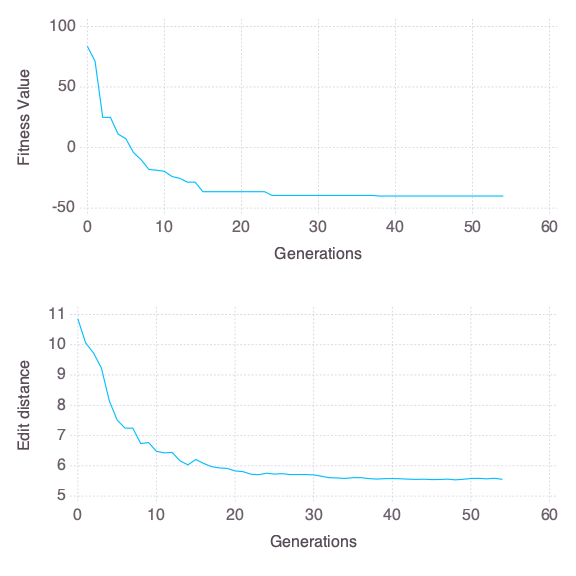
\includegraphics[scale=0.5]{./figures/config_file_10_Rastrigin_diversity.png}
	\caption{ Diversity in the execution with the best fitness value for the Rastrigin function }
    \label{fig:best_restrigin_diversity}
\end{figure}

Now let's compare the entropy for the best and worst execution of the Rastrigin function to see if the entropy has 
anything to do with the algorithm outcome. As we know, algorithms seem to get stuck in local optima when
entropy doesn't change or decrease drably in sequential generations. In Figure \ref{fig:rastrigin_diversity_comparation} we can see
this case in the execution with the worst fitness value. The entropy decreases more thatn 2 points from generation 0 to generation 30.
Whilst in the case of the best execution the entropy slope is less strong. Also in the execution with the best fitness we can see how
when the entropy stays with similar values for multiple generations is when it gets stucked in local optima.

\begin{figure}[]
	\centering	
	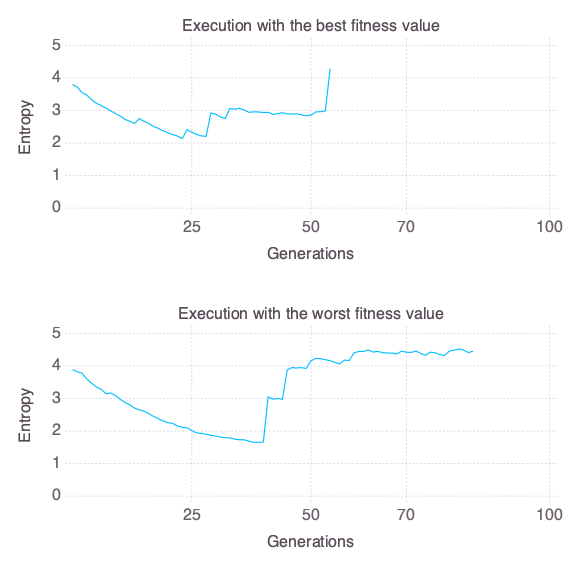
\includegraphics[scale=0.5]{./figures/config_file_10_Rastrigin_diversity_comparation.png}
	\caption{ Comparation of the diversity between the execution with the best and the worst fitness value for the Rastrigin function }
    \label{fig:rastrigin_diversity_comparation}
\end{figure}

With this information we can now compare the diversity of our algorithm with the behaviour of a genetic algorithm without
castes division.

\subsection{Diversity on a basic genetic algoritm}

We will now compare the diversity of the Brave new algorithm with a ``basic`` genetic algorith, meaning an algorithm without castes division, in order
to check how the division affects the diversity.

In Table \ref{tab:diversity_comparation} we can see the results comparation for both algorithms. Having a higher value on
the entropy standard deviation means that the values are spread out over a wider range, this is the case for the Brave
new algorithm. Also, it has a better median of the fitness value. In Figure \ref{fig:rastrigin_diversity_comparation} we can see
how the entropy in the basic algorithm looks like more variant, but the values are only between 5 and 5.5

For this section we can conclude that because the Brave new algorithm has a higher standard deviation on the entropy the 
diversity is mainted throught more generations that for the basic genetic algorithm, resulting in better median for the firness value.

\begin{table}[]
    \centering
    \caption{Entropy results for Brave New Algorithm (BNA) and a genetic algorith without castes division (GA)}
    \begin{tabular}{|c|c|c|c|c|}
    \hline
    \textbf{Algorithm} & \textbf{\begin{tabular}[c]{@{}c@{}}entropy\\ median\end{tabular}} & \textbf{\begin{tabular}[c]{@{}c@{}}f. value\\ median\end{tabular}} & \textbf{entropy $\sigma$} & \textbf{f. value $\sigma$} \\ \hline
    BNA                & 2.9                                                               & -39.56                                                             & 0.41             & 26.12             \\ \hline
    GA                 & 5.27                                                              & 528.21                                                             & 0.01             & 224.09            \\ \hline
    \end{tabular}
    \label{tab:diversity_comparation}
\end{table}

\begin{figure}[]
	\centering	
	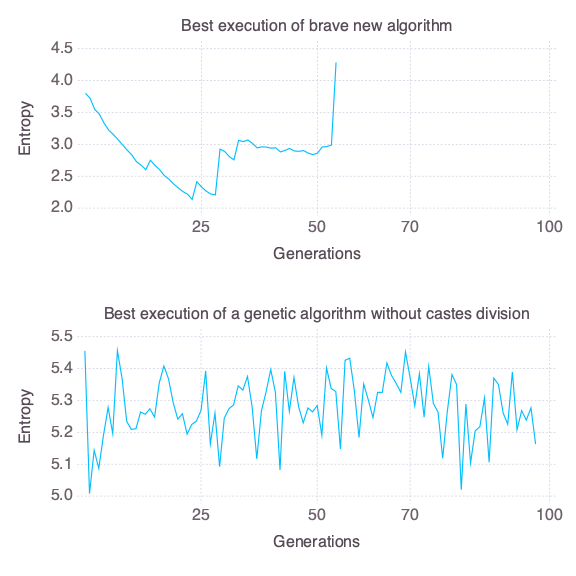
\includegraphics[scale=0.5]{./figures/Rastrigin_diversity_algs_comparation.png}
	\caption{ Comparation of the diversity between the best executions of the Brave New Algorithm and a genetic algorith without castes division }
    \label{fig:diversity_comparation}
\end{figure}


